	\documentclass[10pt,oneside]{CBFT_book}
	% Algunos paquetes
	\usepackage{amssymb}
	\usepackage{amsmath}
	\usepackage{graphicx}
	\usepackage{libertine}
	\usepackage[bold-style=TeX]{unicode-math}
	\usepackage{lipsum}

	\usepackage{natbib}
	\setcitestyle{square}

	\usepackage{polyglossia}
	\setdefaultlanguage{spanish}
	



	\usepackage{CBFT.estilo} % Cargo la hoja de estilo

	% Tipografías
	% \setromanfont[Mapping=tex-text]{Linux Libertine O}
	% \setsansfont[Mapping=tex-text]{DejaVu Sans}
	% \setmonofont[Mapping=tex-text]{DejaVu Sans Mono}

	%===================================================================
	%	DOCUMENTO PROPIAMENTE DICHO
	%===================================================================

\begin{document}

% =================================================================================================
\chapter{Introducción}
% =================================================================================================


% =================================================================================================
\section{El experimento de Stern-Gerlach}
% =================================================================================================

Un horno emite átomos de plata (Ag) neutros con un electrón $e$ en la última órbita que le da el spín
al átomo como un todo. Al salir del horno los átomos tienen su spín orientado en cualquier dirección.
Ver figura.
El momento magnético del átomo que sale del horno es 
\[
	\vb{\mu} = \frac{e}{m_e c} \vb{S}
\]

\begin{figure}[htb]
	\begin{center}
	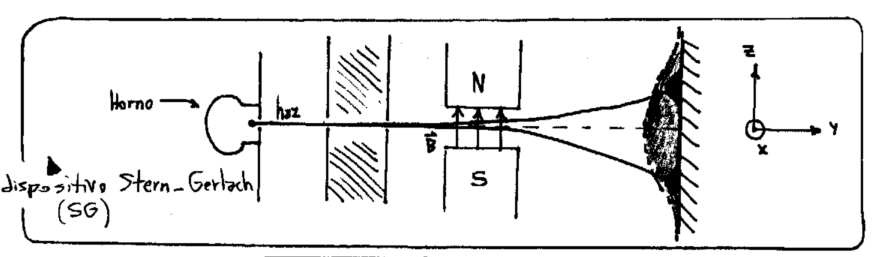
\includegraphics[width=0.8\textwidth]{images/teo2_1.pdf}	 
	\end{center}
	\caption{}
\end{figure} 

La fuerza $f_z$ que le ejerce el campo \vb{B} a estos átomos es 
\[
	f_z \propto - \mu_z
\]
de modo que el dispositivo SG mide y filtra por $S_z(\mu_z)$. Si el spín es un ente clásico
es de esperar un patrón como el sombreado en azul, pero se obtienen dos manchas; con la
correspondencia mostrada bajo estas líneas
\begin{figure}[htb]
	\begin{center}
	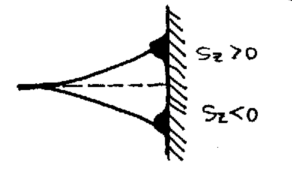
\includegraphics[width=0.4\textwidth]{images/teo2_2.pdf}	 
	\end{center}
	\caption{}
\end{figure} 

Entonces el spín no es un ente {\it continuo}: está cuantizado y sólo puede tomar dos valores.
Llamamos a estos estados
\[
	(S_z,+) \qquad \qquad (S_z,-)
\]
Luego, un aparato de SG filtra o selecciona ciertos átomos. Podemos combinarlos.

\begin{figure}[htb]
	\begin{center}
	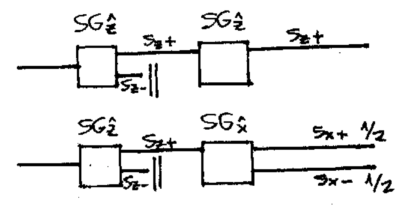
\includegraphics[width=0.6\textwidth]{images/teo2_3.pdf}	 
	\end{center}
	\caption{}
\end{figure} 

Con el dispositivo segundo orientado en $\hat{x}$ obtenemos mitad de átomos en
$(S_z,+)$ y mitad en $(S_z,-)$. La única es que en realidad lo que sucede es que 
$(S_z,+)$ se compone de $(S_x,+)$ y $(S_x,-)$.

Acá abajo sale $(S_z,-)$ pero para que ello sea posible 
$(S_x,+)$ se debe componer de $(S_z,+)$ y $(S_z,-)$. Pero esto no es posible
porque al segundo aparato no entró jamás $(S_z,-)$. Se filtró antes.

Los spines en $S_x, S_z$ son incompatibles. Al seleccionar $(S_z,+)$ en el segundo
SG se destruye la información previa sobre $S_z$. No podemos ya garantizar que $S_z$
sea nula.
El tercer experimento da al traste con la idea de que podamos pensar en spín como un
ente vectorial en 3D. Mediante una analogía con polarización de luz vemos que es necesario
meter al spín es un espacio vectorial de dimensión 2 pero con coeficientes complejos.

\begin{figure}[htb]
	\begin{center}
	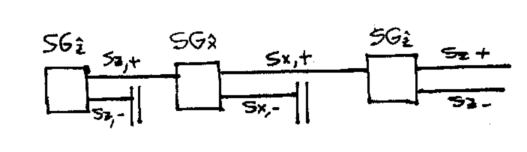
\includegraphics[width=0.6\textwidth]{images/teo2_4.pdf}	 
	\end{center}
	\caption{}
\end{figure} 

% =================================================================================================
\section{Algebra?}
% =================================================================================================

El ket contiene toda la información cuántica del estado. Da el estado físico del sistema.
\begin{itemize}
 \item $\Ket{\alpha} + \Ket{\beta}$ la suma de kets es un ket
 \item $c\Ket{\alpha}= \Ket{\alpha} c$ con $c\in\mathbb{C}$
 \item  $c_1\Ket{\alpha} + c_2\Ket{\beta} = \Ket{\gamma}$ con $c_1,c_2 \in \mathbb{C}$
 \item $c\Ket{\alpha},\Ket{\alpha}$ representan el mismo estado cuántico
\end{itemize}

Se define un espacio de {\it Bra} dual al de "kets" al que se va mediante ``dual conjugado''
\[
	\Ket{a}, \Ket{a'} \Leftrightarrow \Bra{a}, \Bra{a'}
\]
\[
	\Ket{a} + \Ket{b} \leftrightarrow \Bra{a} + \Bra{b} \qquad 
	c\Ket{a} \leftrightarrow c^*\Bra{a}
\]

Se define también un producto interno según
\[
	(\Bra{\alpha})(\Ket{\beta}) \equiv \Braket{\alpha|\beta}
\]
que no es otra cosa que un número complejo. Se puede hacer entonces una equivalencia con los vectores
estándard del álgebra del siguiente modo 
\[
	\text{ket} \sim \text{vector columna} \qquad \Ket{x} = \begin{pmatrix}
	                                                       1 \\
	                                                       0 \\
	                                                      \end{pmatrix}
\]
\[
	\text{bra} \sim \text{vector fila} \qquad \Bra{x} = ( 1 \; 0 )          
\]
y habiendo definido esta base escribimos, por ejemplo
\[
	\Ket{a} = \frac{1}{\sqrt{2}} \begin{pmatrix} 1 \\ 1  \\ \end{pmatrix}  =
	\frac{1}{\sqrt{2}} \begin{pmatrix} 1 \\ 0  \\ \end{pmatrix}  + 
	\frac{1}{\sqrt{2}} \begin{pmatrix} 0 \\ 1  \\ \end{pmatrix} =
	\frac{1}{\sqrt{2}} \Ket{x} + \frac{1}{\sqrt{2}} \Ket{y} 
\]
\[
	\Braket{a|x} = \frac{1}{\sqrt{2}}( 1 \; 1)\begin{pmatrix} 1 \\ 0  \\ \end{pmatrix} = \frac{1}{\sqrt{2}}
\]
y del mismo modo
\[
	\left( \frac{1}{\sqrt{2}} \Bra{x} + \frac{1}{\sqrt{2}} \Bra{y}  \right)
	\left( \Ket{x} \right)= \frac{1}{\sqrt{2}}
\]

\subsection{Propiedades}

\begin{enumerate}
 \item $\Braket{\beta|\alpha} = \Braket{\beta|\alpha}^*$ \text{luego} $ \Braket{\alpha|\alpha} \; \in \mathbb{R}$
 \item $\Braket{\alpha|\alpha} \geq 0$ \text{métrica definida positiva}
 \item $\Braket{\alpha|\beta} = \Braket{\beta|\alpha} = 0 \Leftrightarrow \Ket{\alpha} \perp \Ket{\beta}$
 \item $\Braket{\tilde{\alpha}|\tilde{\alpha}} = 1 \; \text{con} \; 
 \Ket{\tilde{\alpha}} = \frac{1}{\sqrt{\Braket{\alpha|\alpha}}}\Ket{\alpha} $ todo ket no nulo es normalizable
\end{enumerate}

\subsection{Operadores}

A cada observable lo representaremos por un operador. hay operaradores que no vienen de observables.
\[
	\hat{A}\Ket{\alpha} = \Ket{\gamma} \qquad \qquad  \Bra{\alpha} \hat{A} = \Bra{\gamma}
\]
un operador sobre un ket da otro ket y sobre un bra da otro bra. Notemos que en este último caso opera 
a izquierda. La transformación entre operadores se da con 
\[
	\hat{X}\Ket{a} \Leftrightarrow \Bra{a}\hat{X}^\dagger
\]
donde $\dagger$ (daga) significa el traspuesto conjugado; cambia el sentido hacia donde actúa el operador 
y conjuga. Se da que si 
\[
	\hat{X} = \hat{X}^\dagger \quad \Rightarrow \qquad \hat{X} \;\text{es hermítico}
\]
Se dan 
\begin{itemize}
 \item $\hat{X}\hat{Y} \neq \hat{Y}\hat{X} \qquad \qquad \text{no conmutativo}$
 \item $\hat{X}(\hat{Y}\hat{Z}) = (\hat{X}\hat{Y})\hat{Z} = \hat{X}\hat{Y}\hat{Z} \qquad \qquad \text{asociativo}$
 \item $(XY)^\dagger = Y^\dagger X^\dagger$
 \item $\hat{0}\Ket{\alpha} = 0 \qquad \forall \Ket{\alpha}$ ; $\hat{0} \equiv$ operador nulo
 \item $\hat{X}( c_1 \Ket{\alpha} + c_2 \Ket{\beta} ) = c_1 \hat{X}\Ket{\alpha} + c_2 \hat{X}\Ket{\beta} $
\end{itemize}

de modo que en cuántica los observables se representan mediante operadores hermíticos.

\subsection{sandwichs}

\[
	\Braket{\beta|X|\alpha} = (\Bra{\beta})(X\Ket{\alpha}) = \Braket{\beta|\gamma} =
	\Braket{\gamma|\beta}^* = (\Braket{\alpha|X|\beta})^*
\]
donde usamos que $\Ket{\gamma}$ es un ket y por dual conjugado $\Bra{\gamma} = \Bra{\alpha}\hat{X}^\dagger$ y
extraemos como conclusión 
\[
	\Braket{\beta|X|\alpha} = (\Braket{\alpha|X|\beta})^*
\]
y de manera equivalente
\[
	\Braket{\beta|X|\alpha} = (\Bra{\beta}X^\dagger)(\Ket{\alpha}) = \Braket{\Gamma|\alpha} =
	\Braket{\alpha|\Gamma}^* = (\Braket{\alpha|X^\dagger|\beta})^*
\]
donde usamos que $\Bra{\Gamma}$ es un bra y por dual conjugado $\Ket{\Gamma} = \hat{X}\Ket{\beta}$.
El formalismo parece ser consistente. El operador opera sobre un ket/bra y multiplica al otro.


\subsection{Producto externo}

\[
	\Ket{\beta} \Bra{\alpha} \equiv (\Ket{\beta} )( \Bra{\alpha} )
\]
\[
	( \Ket{\beta} \Bra{\alpha} )\Ket{\gamma} = \Ket{\beta} \Bra{\alpha} \Ket{\gamma} =
		\Braket{\alpha|\gamma} \Ket{\beta} , 
\]
de modo que es un operador pues al aplicar sobre un ket obtengo otro ket (notemos que $\Braket{\alpha|\gamma}$
es un escalar). Podemos pensar en que 
\[
	\Lambda_\alpha \equiv \Ket{\alpha}\Bra{\alpha}
\]
es el proyector, que actúa rotando un $\Ket{\gamma}$ en la dirección de $\Ket{\beta}$. Notemos 
\[
	\Lambda_\alpha^2 = \Ket{\alpha}\Bra{\alpha}\Ket{\alpha}\Bra{\alpha} = \Ket{\alpha}\Bra{\alpha} = \Lambda_\alpha
\]
puesto que $\Braket{\alpha|\alpha}=1$. El proyector $\Lambda_\alpha$ sobre un ket $\Ket{\beta}$ selecciona la parte de
$\Ket{\beta}$ en la dirección de $\Ket{\alpha}$. Nos dice cuanto de $\Ket{\beta}$ está en la dirección de 
$\Ket{\alpha}$.
Luego,
\[
	\sum_i^N \; \Lambda_i = \sum_i^N \; \Ket{i}\Bra{i} = \mathbb{1}
\]
la suma de todos los proyectores del espacio en el que estamos es la identidad de ese espacio. Decimos que $\Ket{i}$ es 
un conjunto completo. Se verifica además
\[
	(\Ket{\beta} \Bra{\alpha})^\dagger = \Ket{\alpha} \Bra{\beta}
\]
Algunas cuentitas de ejemplo en dos dimensiones,
\[
	\hat{X} = \begin{pmatrix} 1 \\ 0 \end{pmatrix} \qquad \qquad \hat{Y} = \begin{pmatrix} 0 \\ 1 \end{pmatrix}
\]
\[
	\hat{X}^\dagger = ( 1 \; 0 ) \qquad \qquad \hat{Y}^\dagger = ( 0 \; 1  ) 
\]
\[
	\hat{X}^\dagger\hat{X} = (1 \; 0) \begin{pmatrix} 1 \\ 0 \end{pmatrix} = 1 \qquad 
	\hat{X}\hat{X}^\dagger = \begin{pmatrix} 1 \\ 0 \end{pmatrix} (1 \; 0) = 
	\begin{pmatrix} 1 & 0 \\ 0 & 0 \\ \end{pmatrix},
\]
donde instamos al lector a que note la diferencia de dimensión en los resultados.

Los kets $\Ket{\alpha}$ {\it viven} en un espacio vectorial de Hilbert con dimensión N, donde N lo dicta el número de 
posibles estados de cada sistema físico. Una partícula de spín $1/2$ sólo tiene dos estados: up y down.
Hay otro producto más, que se llama producto tensorial y se representa como 
\[
	\Ket{\alpha} \otimes \Ket{\beta}
\]
que es un producto entre kets de espacios de Hilbert diferentes.
\[
	\Braket{\alpha|\beta}^* \equiv DC\{\ket{\beta}\} DC\{\Bra{\alpha}\}
\]

\section{Bases}

Dado un sistema físico representado por un espacio vectorial $\mathcal{H}$ de dimensión $N$ existirá una base (también 
de dimensión $N$) que será un conjunto de estados tal que cualquier estado de ese sistema físico puede representarse 
como combinación lineal de ese conjunto,
\[
	\{ \Ket{i}\} \; \text{base} \quad \Rightarrow \; \Ket{\alpha} = \sum_i^N c_i \Ket{i}
\]
siendo $\Ket{\alpha}$ un estado cualquiera.
Es práctico utilizar bases ortonormales,
\[
	\Braket{ i|j } = \delta_{ij} = \begin{cases}
	                                1 \quad i=j \\
	                                0 \quad i\neq j
	                               \end{cases}
\]
que es la delta de Kronecker.

Así, los kets se definen normalizados.
\[
	\Ket{\psi} = a \Ket{1} + b \Ket{2} + c \Ket{3} + d \Ket{4} \qquad\quad |a|^2 + |b|^2 +|c|^2 +|d|^2 = 1
\]
sea $\Ket{\phi} = a \Ket{1} + b \Ket{2}$, $\Bra{\phi} = a^*\Bra{1} + b^* \Bra{2}$ entonces 
\[
	\Braket{\phi|\phi} = (a^*\Bra{1} + b^* \Bra{2})(a \Ket{1} + b \Ket{2}) = 
	a^*a \Braket{1|1} + b^*a\Braket{2|1} + a^*b\Braket{1|2} + b^*b\Braket{2|2} =
	|a|^2 + |b|^2 = 1
\]

\subsection{Autokets y autovalores}

Si $\hat{A}\Ket{a}=c\Ket{a}$ entonces $\Ket{a}$ es autoket de $\hat{A}$ con autovalor $c$. Se suelen 
etiquetar los autoestados $\Ket{a'}, \Ket{a''}$ de modo que 
\[
	\hat{A}\Ket{a'} = a'\Ket{a'}
\]
lo cual lleva al problema espectral
\[
	\left(\hat{A} - a'\mathbb{1}\right) \Ket{a'} = 0
\]
entonces los operadores tendrán representación matricial, que cambiará según la base utilizada.ñ
Vamos viendo que en general sólo se sabe cómo opera un operador sobre kets. La operación sobre los
bras la obtenemos usando dual conjugado.

Deducimos entonces que 



% \bibliographystyle{CBFT-apa-good}	% (uses file "apa-good.bst")
% \bibliography{CBFT.Referencias} % La base de datos bibliográfica

\end{document}
